\section{Comparisons}
This section contains several different comparisons between the different runs to illustrate performance properties of each algorithm. 

\subsection{Making the Comparisons}
Each run of the two algorithms can contain designs that were exposed to numerous different load cases across the possible input space. Additionally, the design results between the Stochastic Loads and the Aggregated LHS methods are not comparable natively. 

To overcome this inconsistency between the different runs, additional processing was required. The designs from each run were re-analyzed using a single, common reference load of: 
\begin{align*}
P_x &=0 &P_y &= -150 \; \text{kN}
\end{align*}
Once the analysis was completed, the peak stress was obtained for each design. Because the load case used to make the data is different from the earlier sections, the stress responses may appear inconsistent with the previous graphs. However, this is due to the change in loading, not because the designs have changed. 

Additionally, The reliability index for all designs was calculated for all designs using the exact same methods indicated in section \ref{sec:beta}. This data was also plotted for each run. 

\subsection{Comparison of Long Run Results}
Figures \ref{fig:pfront_comp_long} and \ref{fig:pfront_comp_long} show plots of this comparison between the two Long-Run fronts. Note that the solver for the aggregate LHS appears to cover a wider portion of the solution space, but that both graphs follow roughly the same curve. 

\begin{figure}[!htbp]
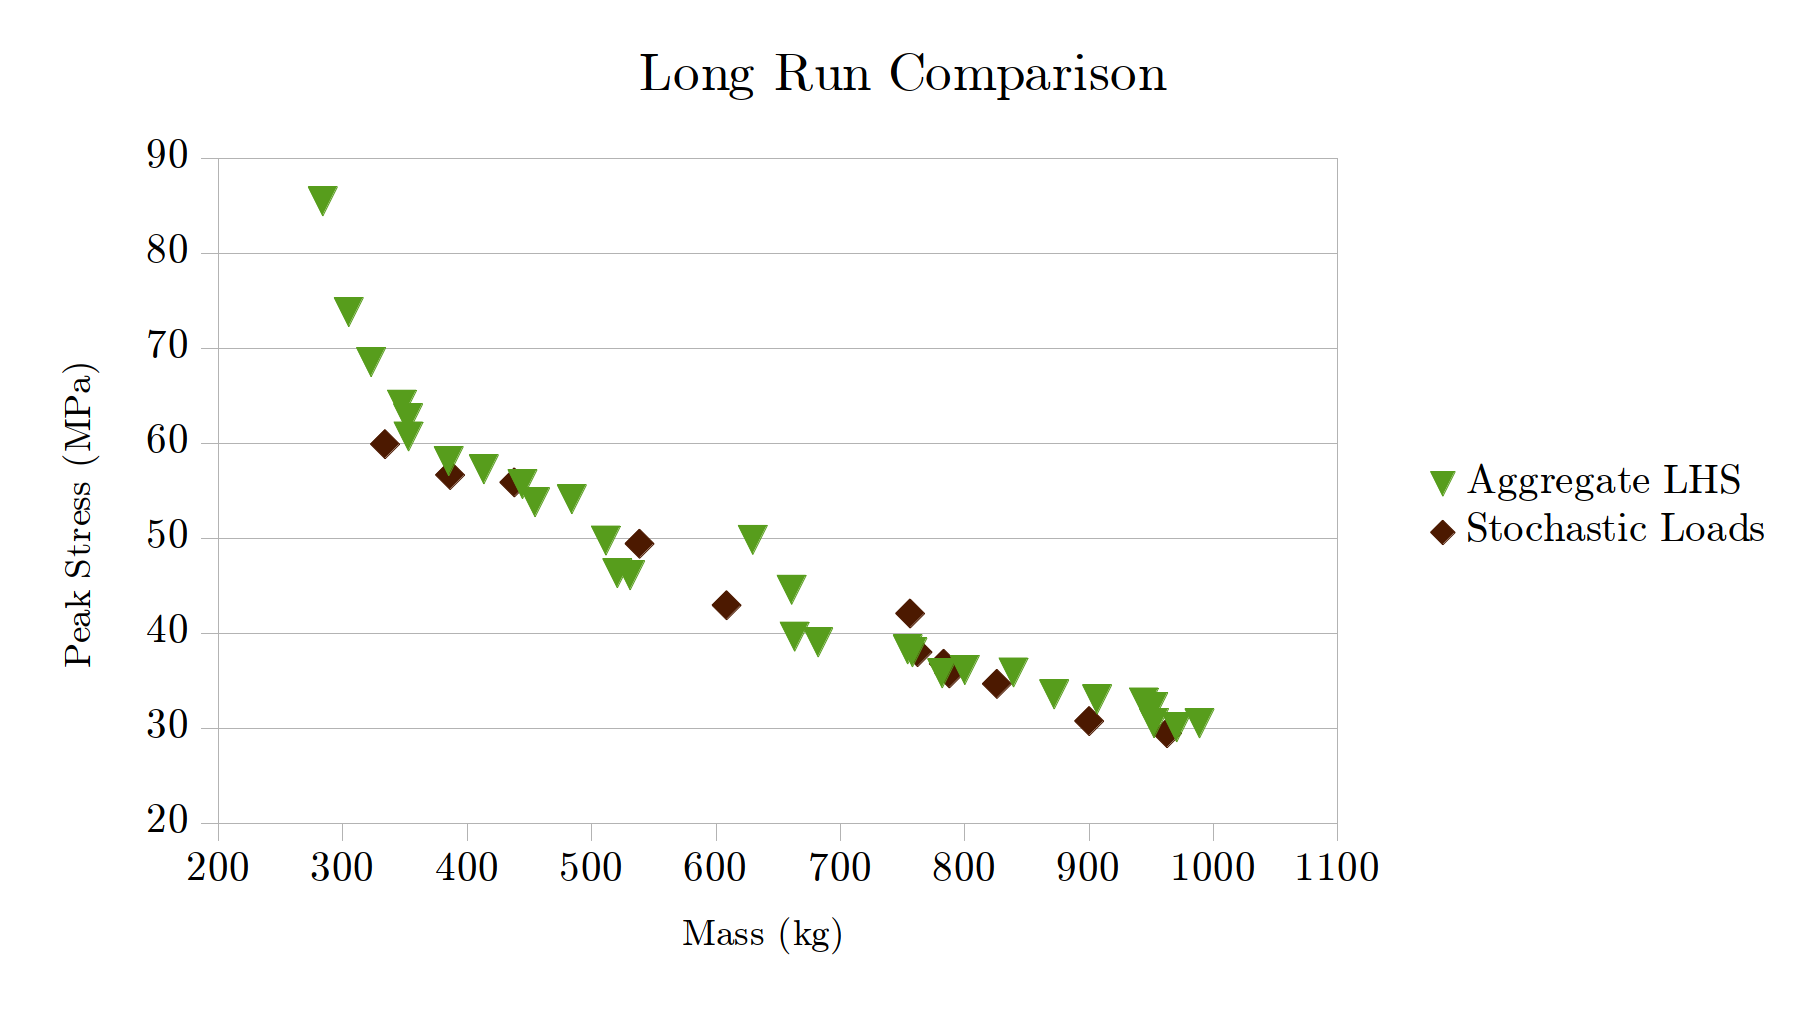
\includegraphics[width=\textwidth]{img/pf_comp_long.png}
\caption{Peak Stress Comparison of the Two Long Run Pareto Plots}
\label{fig:pfront_comp_long}
\end{figure}

\begin{figure}[!htbp]
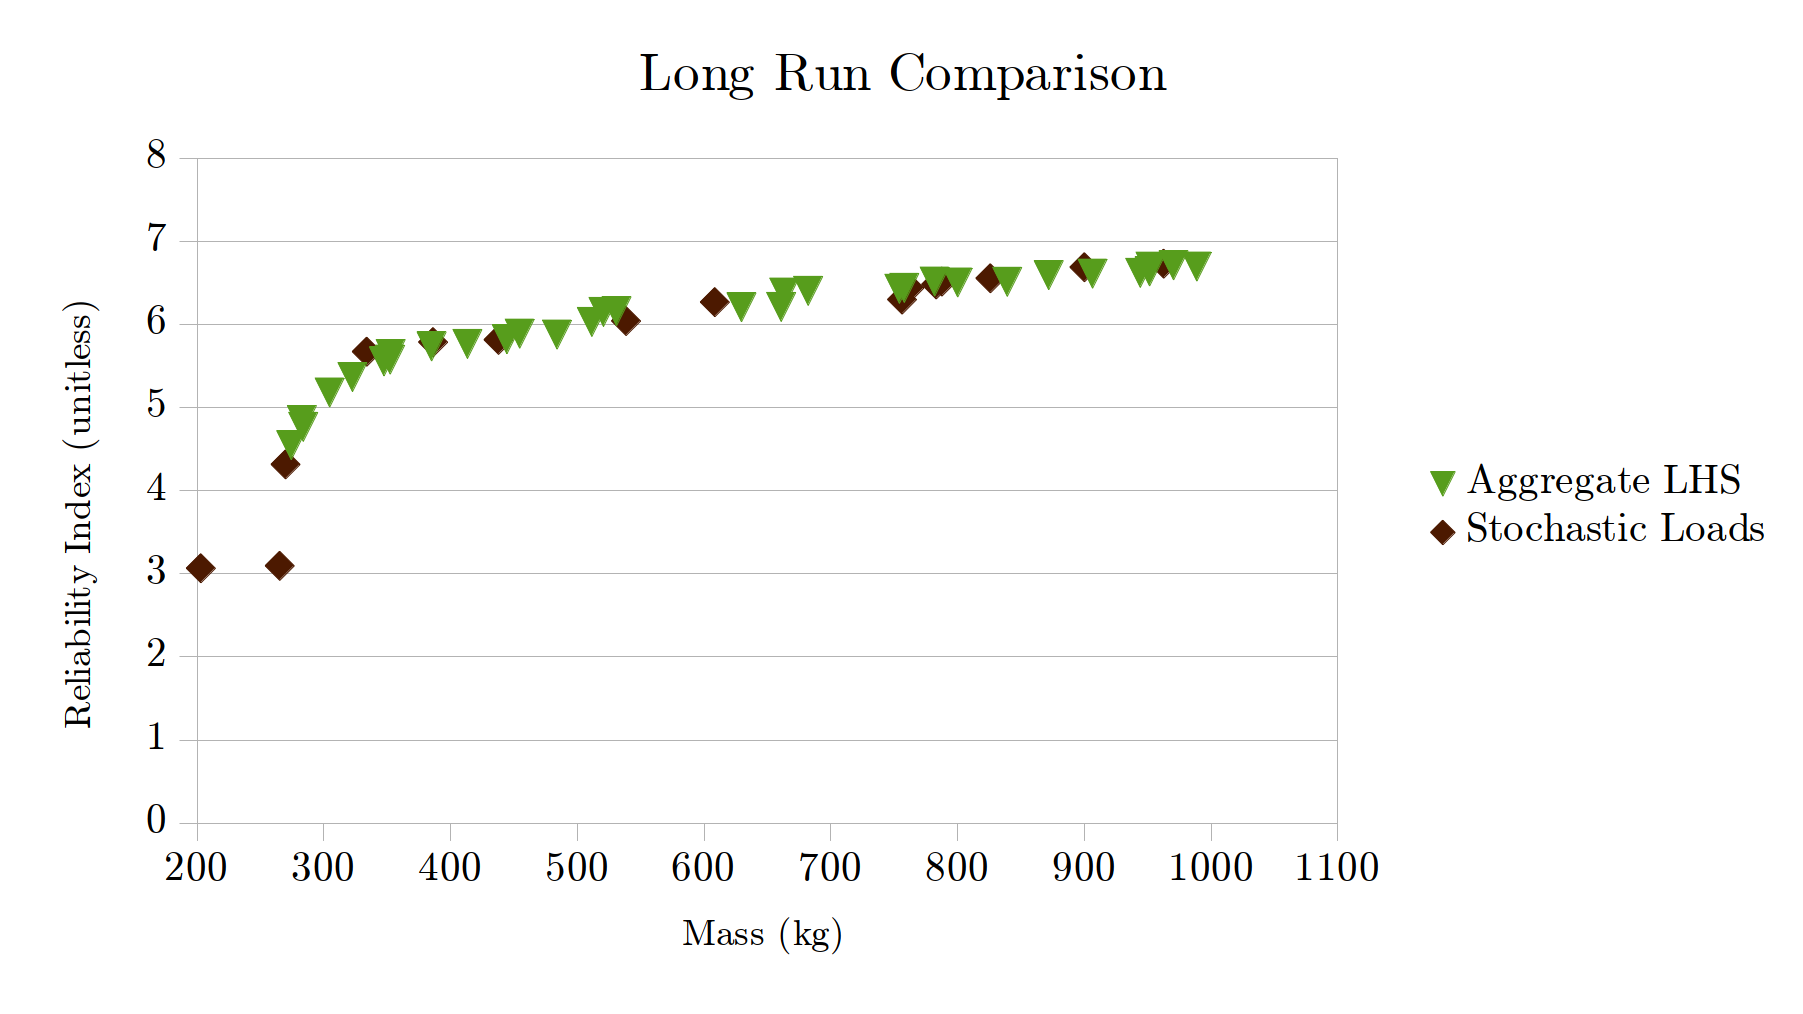
\includegraphics[width=\textwidth]{img/pf_comp_long_beta.png}
\caption{Reliability Index Comparison of the Two Long Run Pareto Plots}
\label{fig:pfront_comp_long_beta}
\end{figure}

\subsection{Comparison of Intermediate Run Results}
Figures \ref{fig:pfront_comp_int} and \ref{fig:pfront_comp_int_beta} show plots of the comparison between the two Intermediate-Run fronts. Note that the solver for the aggregate LHS appears to have slightly better performance at lighter weights than Stochastic Loads. 

\begin{figure}[!htbp]
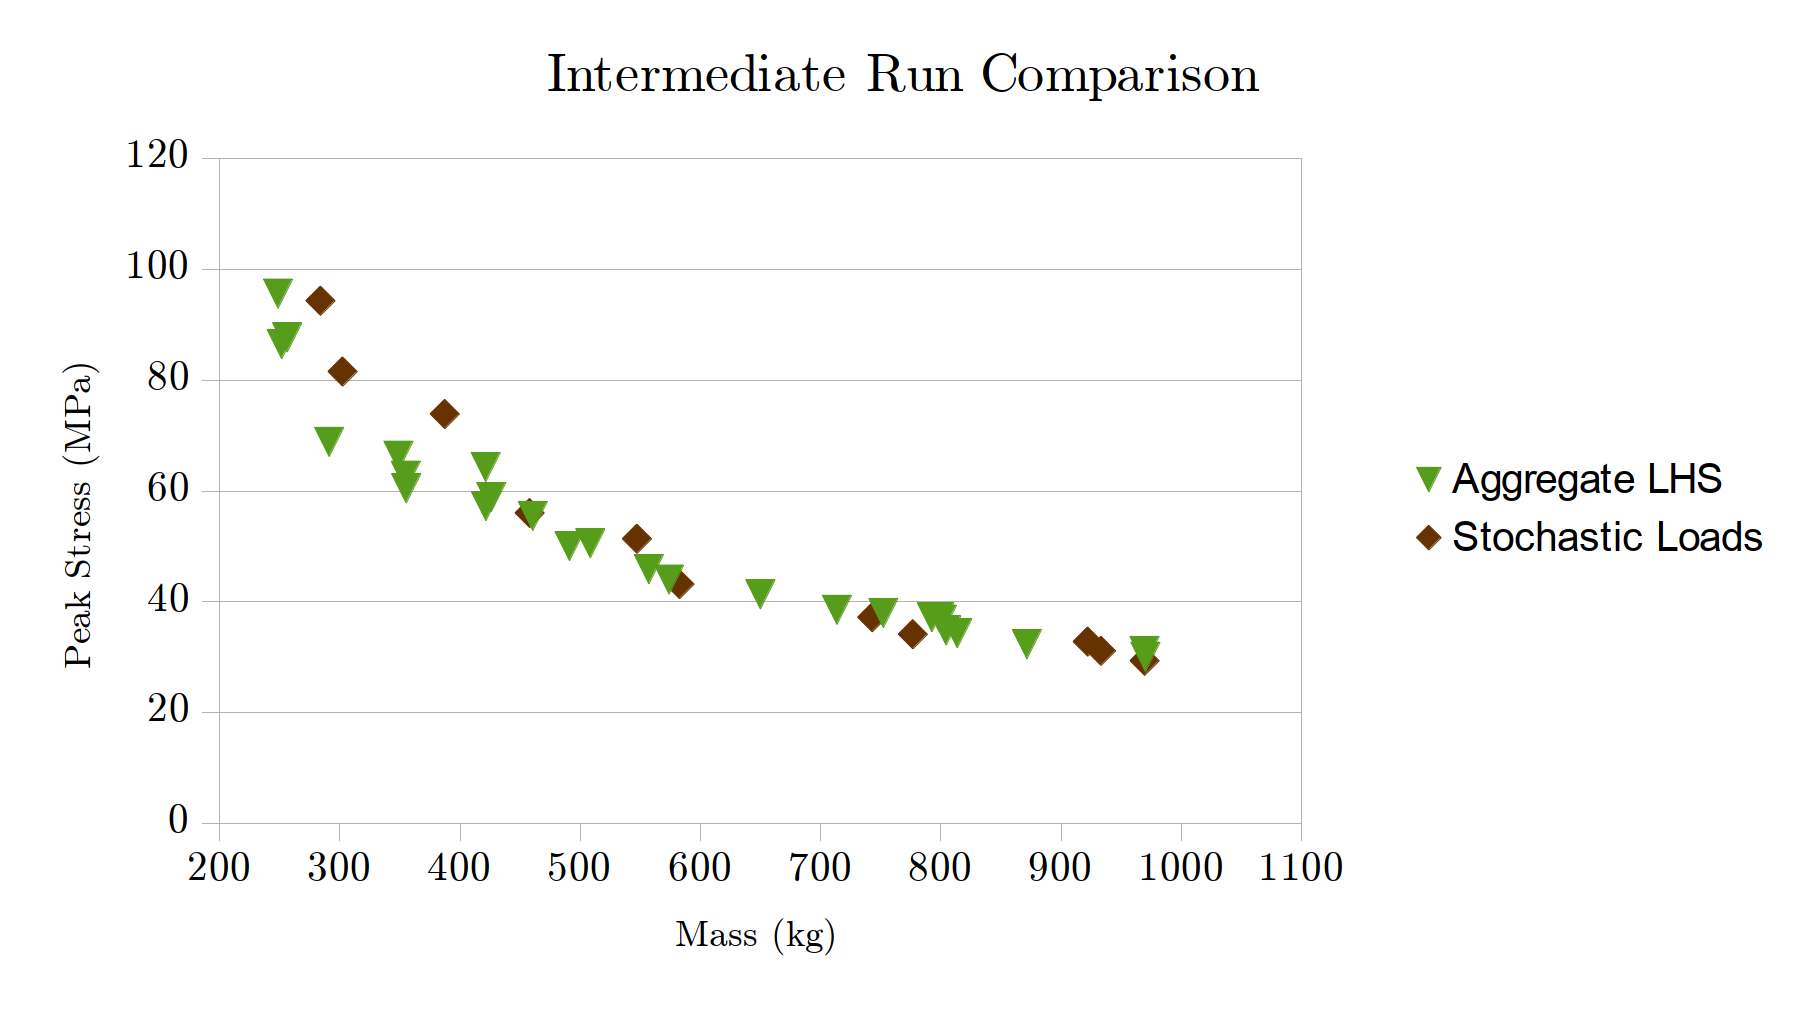
\includegraphics[width=0.9\textwidth]{img/pf_comp_int.png}
\caption{Peak Stress Comparison of the Two Intermediate Run Pareto Plots}
\label{fig:pfront_comp_int}
\end{figure}
\begin{figure}[!htbp]
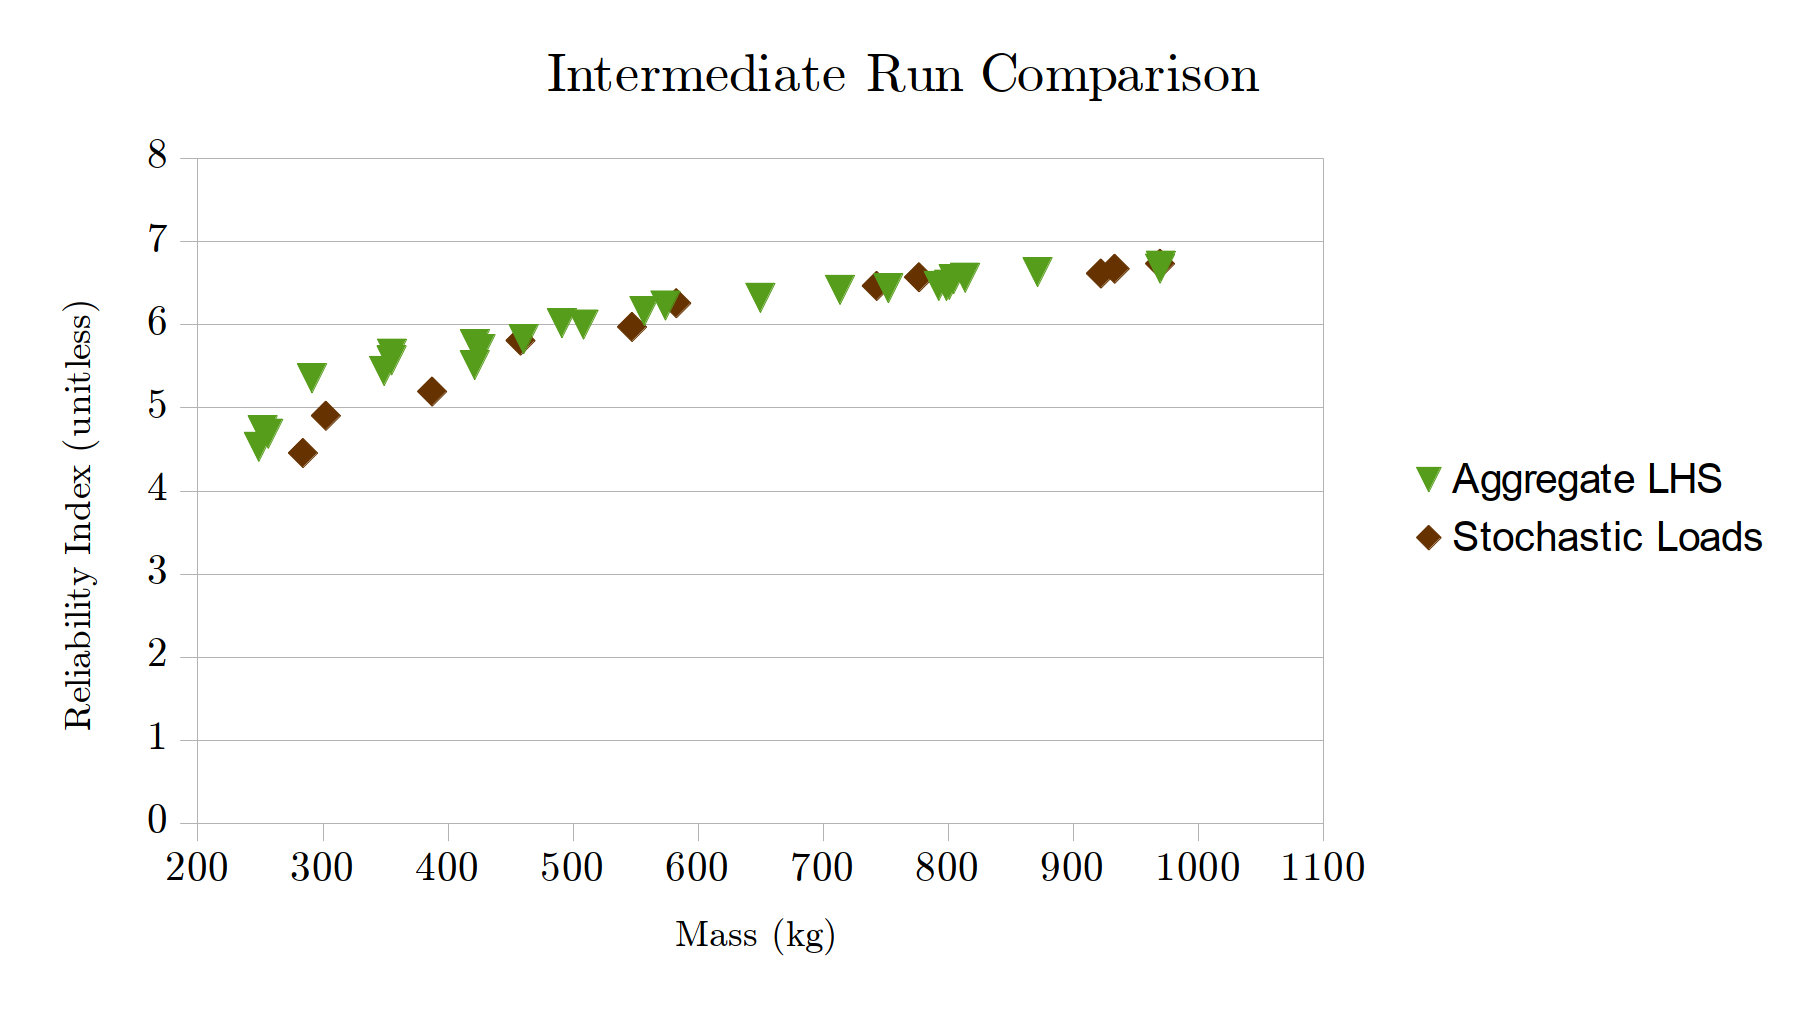
\includegraphics[width=0.9\textwidth]{img/pf_comp_int_beta.png}
\caption{Reliability Index Comparison of the Two Intermediate Run Pareto Plots}
\label{fig:pfront_comp_int_beta}
\end{figure}

\subsection{Comparison of Short Run Results}
Figures \ref{fig:pfront_comp_short} and \ref{fig:pfront_comp_short_beta} show plots of the comparison between the two Short-Run fronts. Note that despite the same solution times, the Stochastic Loads plot has resulted in designs returning higher stress values in some weight ranges. 

\begin{figure}[!htbp]
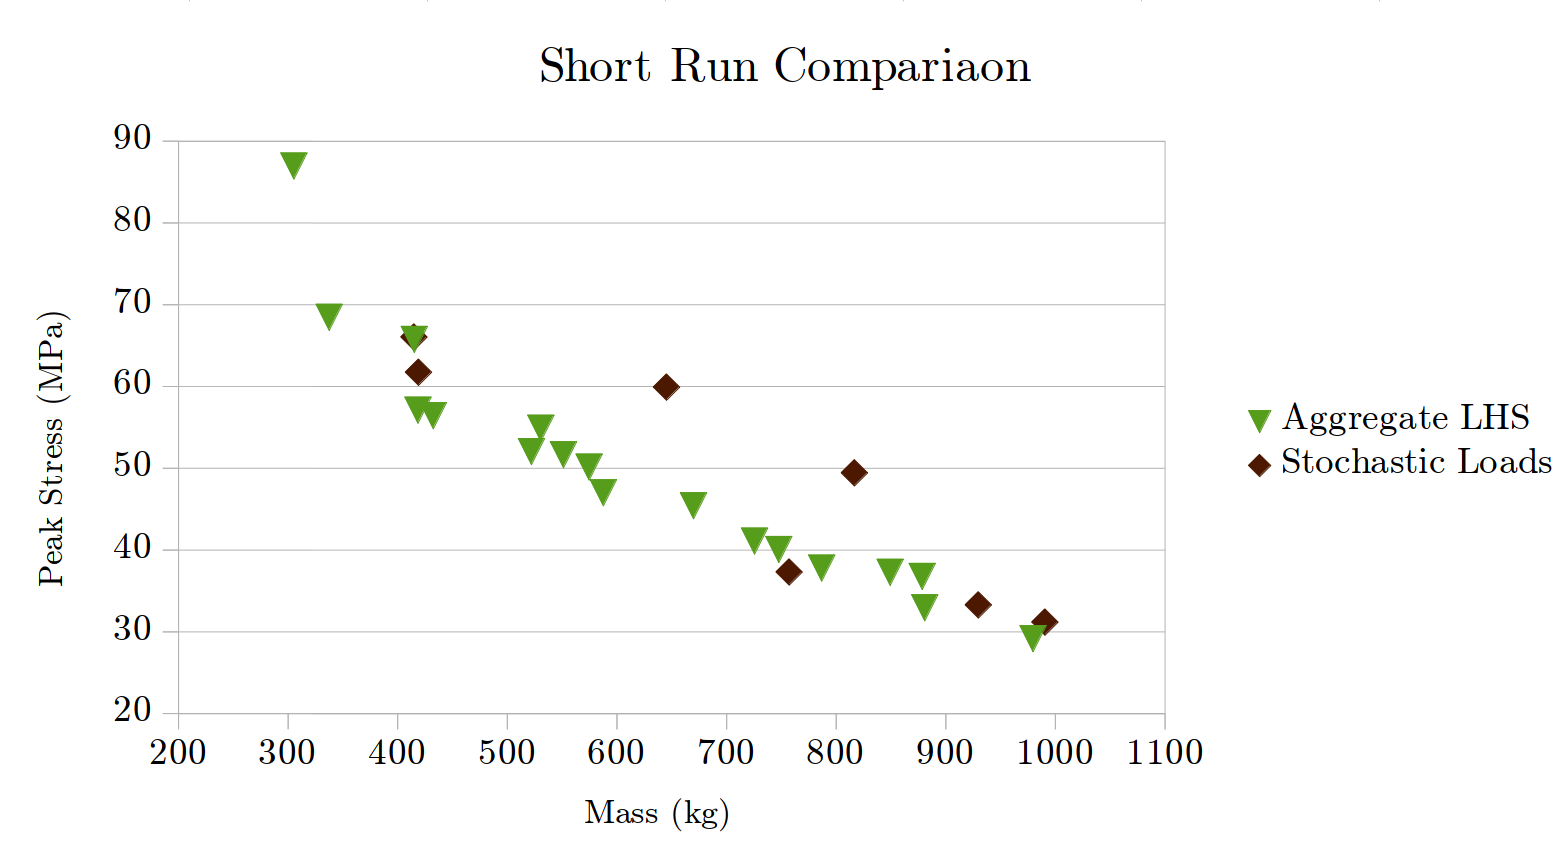
\includegraphics[width=0.9\textwidth]{img/pf_comp_short.png}
\caption{Peak Stress Comparison of the Two Short Run Pareto Plots}
\label{fig:pfront_comp_short}
\end{figure}

\begin{figure}[!htbp]
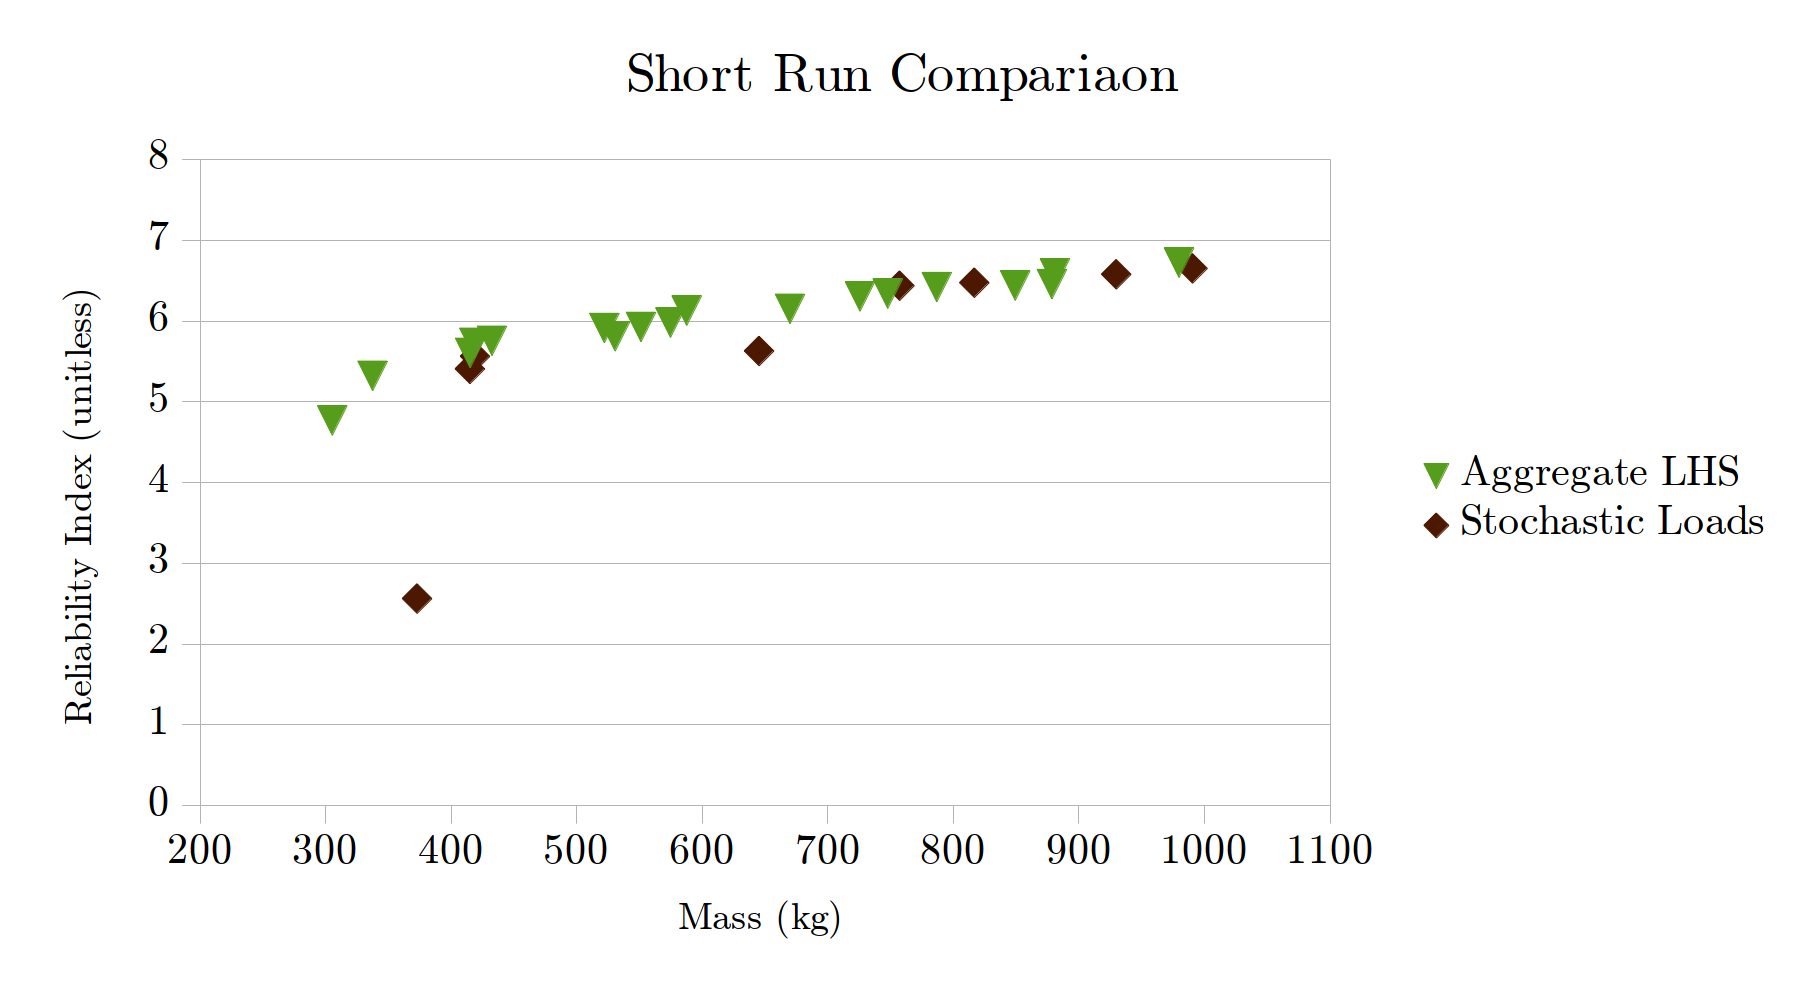
\includegraphics[width=0.9\textwidth]{img/pf_comp_short_beta.png}
\caption{Reliability Index Comparison of the Two Short Run Pareto Plots}
\label{fig:pfront_comp_short_beta}
\end{figure}
\subsection{Comparison of All Stochastic Loads Plots}
Figure \ref{fig:pfront_comp_sto} shows a plot of this comparison between the three Stochastic Loads fronts. Note the increase in accuracy as the solution time rises. 

\begin{figure}[!htbp]
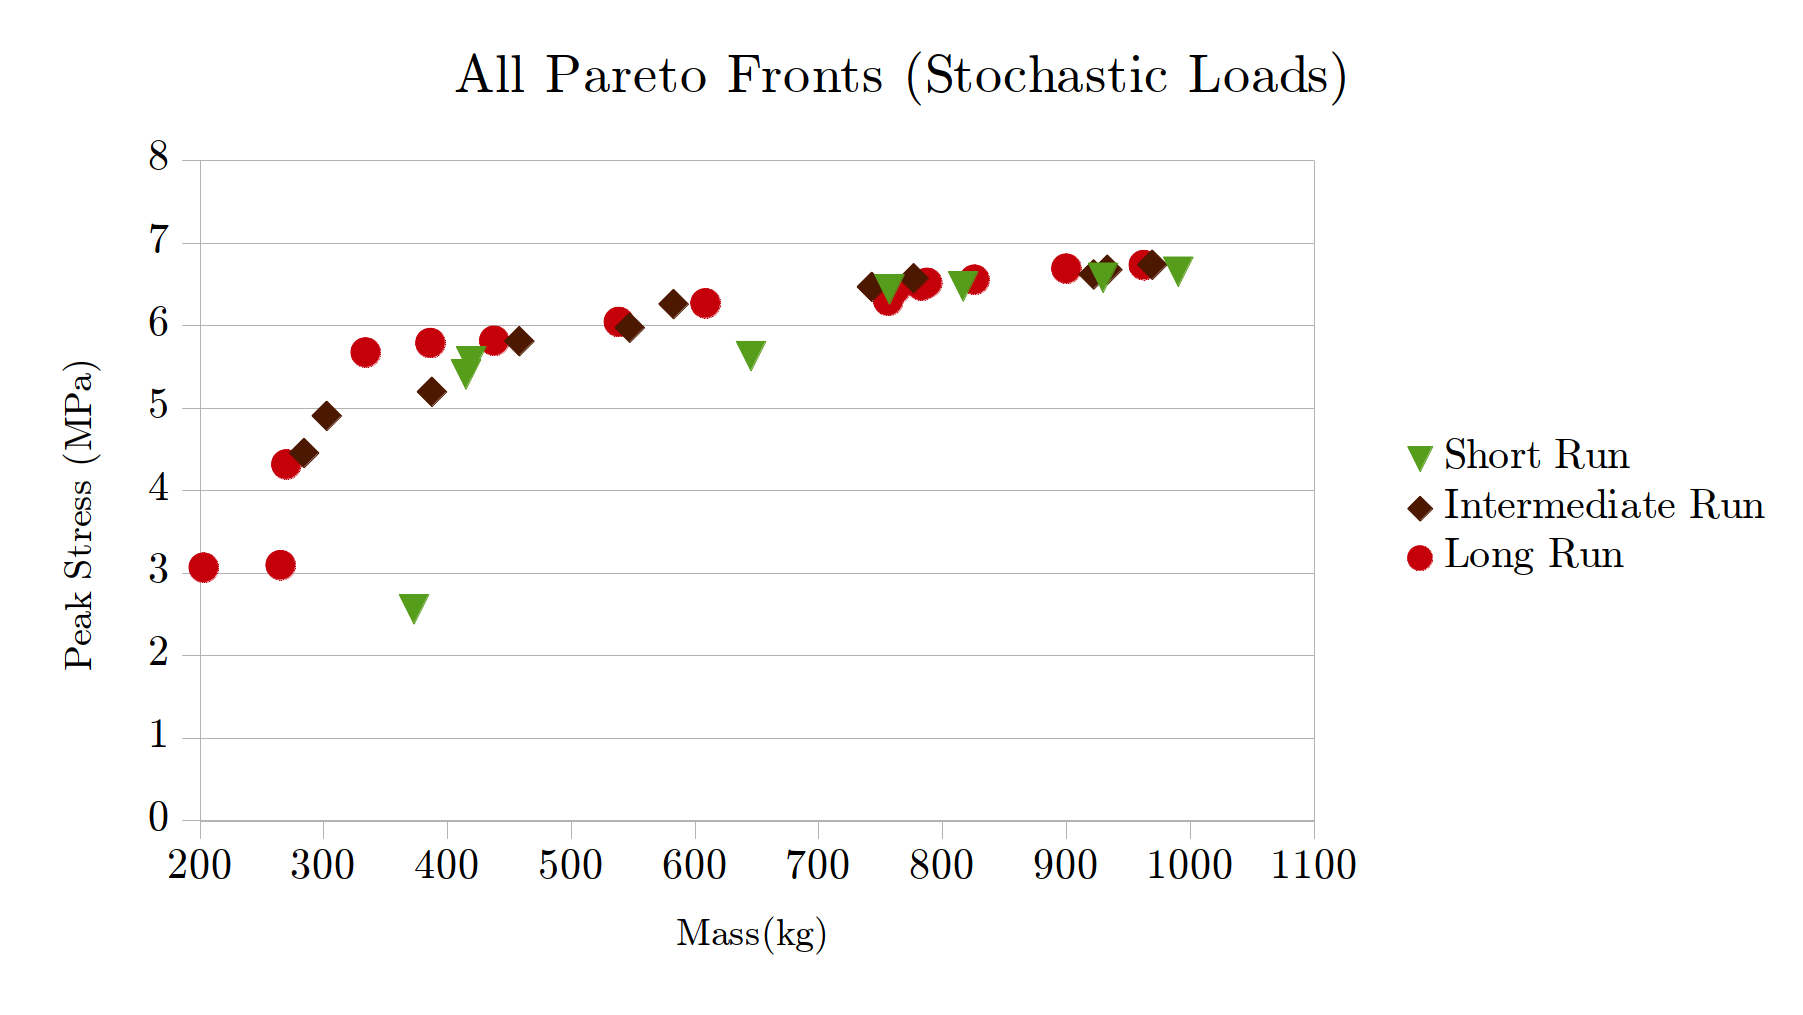
\includegraphics[width=0.9\textwidth]{img/pf_comp_sto.png}
\caption{Comparison of the Stochastic Loads Pareto Plots}
\label{fig:pfront_comp_sto}
\end{figure}

\subsection{Comparison of All Aggregate LHS Plots}
Figure \ref{fig:pfront_comp_agg} shows a plot of this comparison between the three Aggregate LHS fronts. Note the increase in accuracy as the solution time rises, with the exception that the intermediate run seems to have performed better at lighter weights. 

\begin{figure}[!htbp]
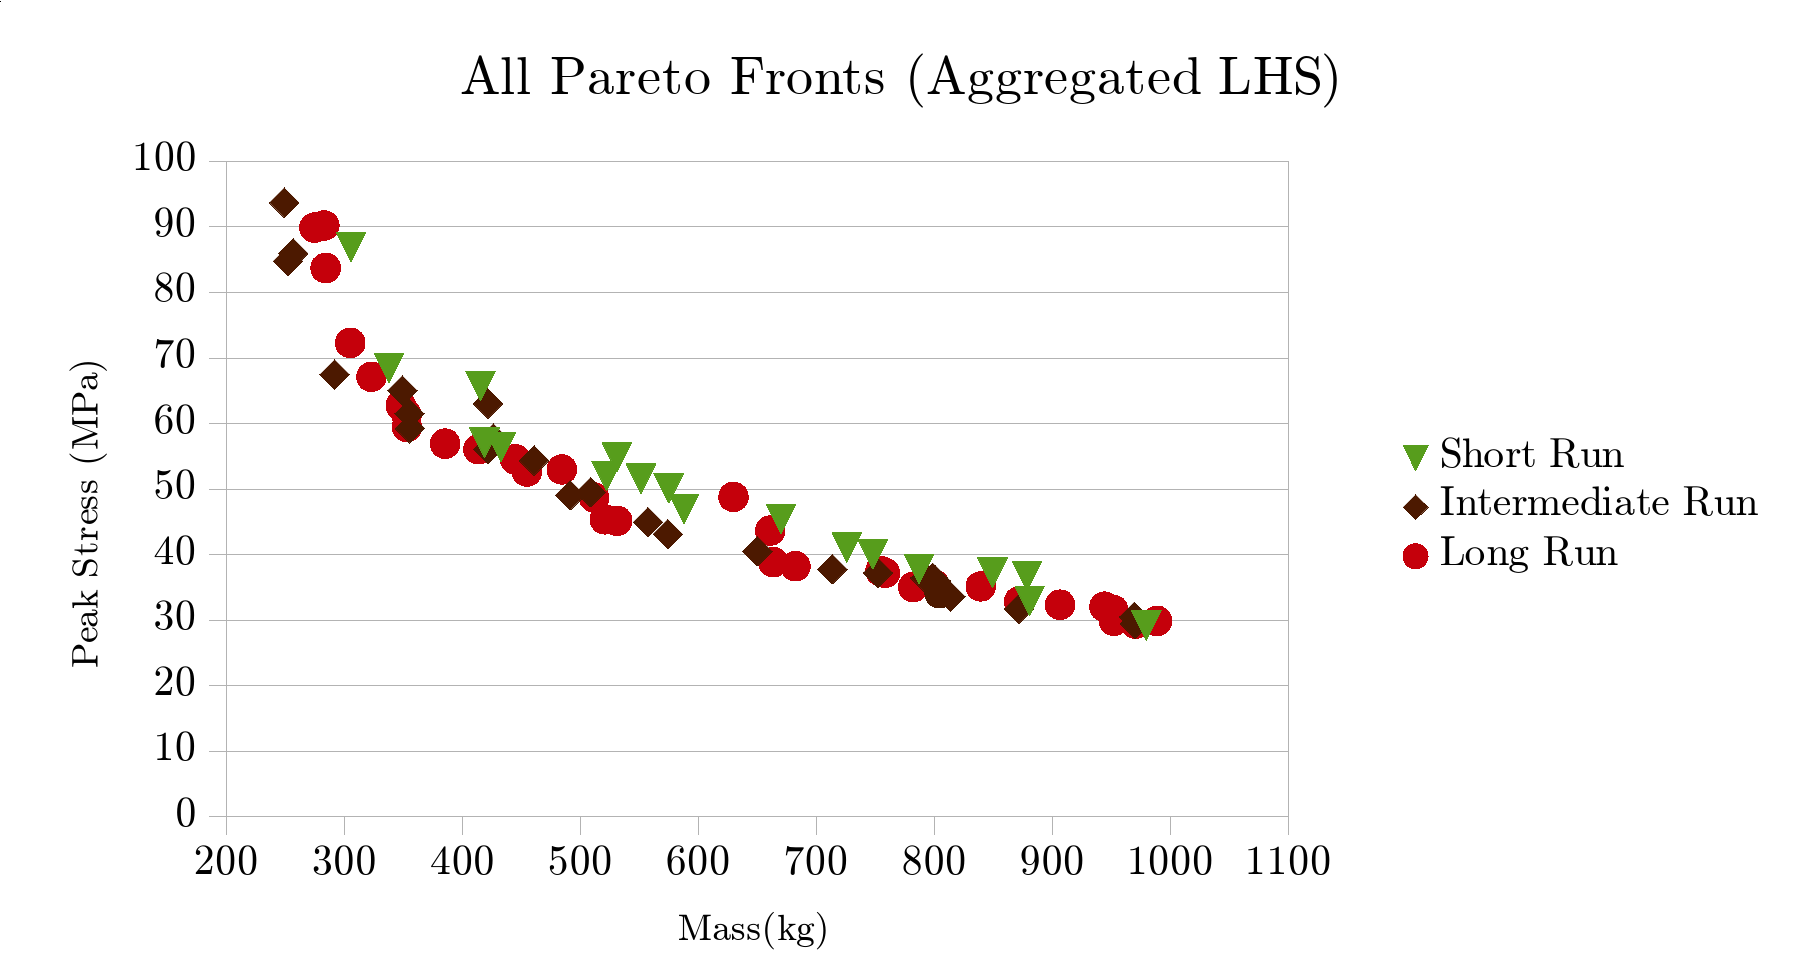
\includegraphics[width=0.9\textwidth]{img/pf_comp_agg.png}
\caption{Comparison of the Aggregate LHS Pareto Plots}
\label{fig:pfront_comp_agg}
\end{figure}

\subsection{Comparison of Run Metrics}
Table \ref{tab:metrics} shows a comparison of all of the collected run metrics for the different runs presented here. Note the particular differences in per-generation times, as well as the number of calls to NASTRAN. 


\begin{table}[!htbp]
\caption{Comparison of Run Metrics for All Runs}
\label{tab:metrics}
\begin{center}
\footnotesize
\begin{tabular}{|l|l|l|l||l|l|l|}
\hline
                            & \multicolumn{3}{|c||}{Stochastic Loads}     & \multicolumn{3}{|c|}{Aggregated LHS}       \\
\hline
                            & Short Run & Intermediate Run & Long Run  & Short Run & Intermediate Run & Long Run  \\
\hline
Individuals Per Generation  & 30        & 80               & 80        & 20        & 80               & 80        \\
Generations Computed        & 25        & 118              & 200       & 2         & 10               & 17        \\
Time Per Generation (sec)   & 18.1      & 44.6             & 44.6      & 205       & 530              & 510       \\
Calls to NASTRAN            & 1.50E+03  & 18.90E+03        & 32.00E+03 & 1.00E+03  & 20.00E+03        & 34.00E+03 \\
Total Wall Clock Time (sec) & 453       & 5.26E+03         & 8.92E+03  & 411       & 5.30E+03         & 8.66E+03  \\
\hline 
\end{tabular}
\end{center}
\end{table}
